%% Road to VPhO 2023 Template

\documentclass[12pt]{article}
\usepackage[utf8]{vietnam}
%\usepackage[english]{babel}
\usepackage[T5]{fontenc}
\usepackage[top=2cm, bottom=2cm, left=2cm,right=2cm]{geometry} %%%% Margin %%%%%
\usepackage[dvipsnames]{xcolor}
\usepackage[pdftex]{graphicx}
\usepackage{wrapfig}
\usepackage{tcolorbox}
\usepackage{mathtools}
\usepackage{amsmath}
\usepackage{amssymb}
\usepackage{eqnarray}
\usepackage{siunitx}
\usepackage{subcaption}
\usepackage{array, lipsum, bibentry,fancyhdr}
\usepackage{hyperref}
\usepackage{natbib}
\setlength{\parindent}{0pt}
\usepackage{enumitem}
\usepackage[noframe]{showframe}
\usepackage{framed}
\usepackage{titling}
\usepackage{float}
\usepackage{multicol}
\usepackage{url}
\usepackage{authblk}
\usepackage{sectsty}
\usepackage{eqparbox}
\usepackage{ulem} 
\usepackage{multirow}

%%%%%%%%%% Pictures drawing %%%%%%%%%%%%%

\usepackage{pgfplots} %%%%%% Regression %%%%
\pgfplotsset{compat = newest}
\usepackage{pgfplotstable}
\usepackage{tikz}
\usepackage{tikz-3dplot} %%%%%% Draw %%%%%%
\usepackage{tikz,tkz-euclide}
\usetikzlibrary{arrows,calc,patterns}
\usetikzlibrary{quotes,angles}
\usetikzlibrary{shapes.geometric}
\usepackage{circuitikz} %%%%% Circuit %%%%
\usetikzlibrary{decorations.pathmorphing,patterns}

\setlength{\unitlength}{1cm}

%%%%%%%%%% Hyperlink %%%%%%%%%%%%%

\hypersetup{
	colorlinks=true,
	linkcolor=black,
	filecolor=mangeta,      
	urlcolor=blue,
	pdftitle={Overleaf Example},
	pdfpagemode=FullScreen,
}


%%%%%%%%%% Set Counter and Reference Equation %%%%%%%%%%

\usepackage{xassoccnt}
\newcounter{totalequations}
\DeclareAssociatedCounters{equation}{totalequations}
\let\theOldHequation\theHequation
\renewcommand{\theHequation}{\theOldHequation::\number\value{totalequations}}


%%%%%%%%%% Header & Footer %%%%%%%%%%%%%

\setlength{\headheight}{10mm}
\RequirePackage{fancyhdr}  % Needed to define custom headers/footers
\RequirePackage{lastpage}  % Number of pages in the document
\pagestyle{fancy}          % Enables the custom headers/footers
% Headers
\lhead{
\includegraphics[width=.8in]{xPhO.png}}%
\chead{}%
\rhead{\small\sffamily\bfseries{Hướng tới chuyên lý 2024} --- \thepage/\pageref{LastPage}}
% Footers
\lfoot{}%
\cfoot{}%
\rfoot{}%
\renewcommand{\headrulewidth}{1pt}% % header rule
\renewcommand{\footrulewidth}{1pt}% % footer rule

% \pagestyle{fancy}
% 	\fancyhead[L]{\empty}
% 	\fancyhead[R]{\empty}
% 	\fancyhead[C]{\empty}
% 	\fancyfoot[C]{\empty}
% 	\fancyfoot[L]{\empty}
% 	\renewcommand{\headrulewidth}{0pt}
% 	\fancyfoot[C]{\normalcolor{\thepage/\pageref{LastPage}}}
% 	\setcounter{page}{1}

%%%%%%%%%% Color setup %%%%%%%%%%%%%

\RequirePackage{xcolor}
\definecolor{wsdred}{HTML}{8E1728}
\definecolor{wsdgrey}{HTML}{75787B}
\definecolor{battleshipgrey}{rgb}{0.52, 0.52, 0.51}
\renewcommand{\normalcolor}{\color{wsdred}}
\colorlet{ColorOr}{white}

\begin{document}

%% Title %%
{\fontsize{50}{24}\fontfamily{phv}\fontseries{b}
\LARGE \normalcolor{ \textbf{Hướng tới chuyên lý 2024} } }

\textcolor{blue}{\textbf{Câu lạc bộ vật lý xPhO}}
%%%%
\vspace{5mm}

{\normalcolor\textbf{CÂU 1}}\vspace{1.5mm}

\setcounter{equation}{0}
Một chiếc thanh mảnh có độ dài $L$ và trọng lượng $P$ phân bố đều. Thả thanh vào một chất lỏng có trọng lượng riêng gấp $\gamma$ lần trọng lượng riêng của thanh (với $\gamma>1$), rồi nhấc một đầu thanh lên bằng một lực kéo $T$ theo phương thẳng đứng với độ lớn có thể điều chỉnh được sao cho thanh nằm cân bằng và nghiêng một góc $\alpha$ so với phương thẳng đứng sao cho $0^\circ<\alpha< 90^\circ$. 

%Gia tốc trọng trường là $g$. 

%\footnote{Thông thường, ở trái đất, gia tốc trọng trường là $g= \SI{9.81}{m/s^2} \approx \SI{10}{m/s^2}$. Số $10$ này chính là số 10 trong công thức liên hệ giữa trọng lượng $P$ và khối lượng $m$, tức là ta có thể viết $P=mg$ thay vì $P=10m$.}

\begin{center}
\begin{tikzpicture}[scale=1]
    \filldraw[color=white, fill=cyan!40] (-3,-1.2) rectangle (3,1.2);
    \draw[ultra thick] (-1,-0.4)--(1,2.6);
    \draw[dashed] (0,0.4)--(0,2);
    \draw (0.25,1.5) arc (60:90:0.5);
    \draw (0.2,1.5) node[above]{$\alpha$};
    \draw[dashed] (1,2.6)--(2,2.6);
    \draw[<->] (2,2.6)--(2,1.2);
    \draw (2,1.9) node[right]{$h$};
    \draw (2.7,-1.2) node[left,above]{$\gamma$};
    \draw[->] (1,2.6)--(1,3.4);
    \draw (1,3) node[right]{$\Vec{T}$};
\end{tikzpicture}
\end{center}

\begin{enumerate}[label=\textbf{\alph*,}]\itemsep0em
    \item Ban đầu $\alpha=\alpha_0$, thanh nằm cân bằng, độ cao đầu trên của thanh so với mặt nước là $h$. Tính $\alpha_0$ theo $\gamma$, $h$, $L$ và tìm điều kiện của $h$ theo $\gamma$, $L$ để thỏa mãn điều kiện $0^\circ < \alpha_0 < 90^\circ$.
    \item Dùng lực $T$ kéo chậm thanh khỏi mặt nước. Tìm công của lực kéo $T$ để kéo vật từ khi thanh nằm nghiêng góc $\alpha_0$ đến khi thanh vừa được kéo hoàn toàn ra khỏi mặt nước, biểu diễn kết quả theo $P$, $L$, $\gamma$ và $\alpha_0$.
\end{enumerate}




\newpage

{\normalcolor \textbf{CÂU 2}}\vspace{1.5mm}

\setcounter{equation}{0}
\begin{figure}[ht]
\centering
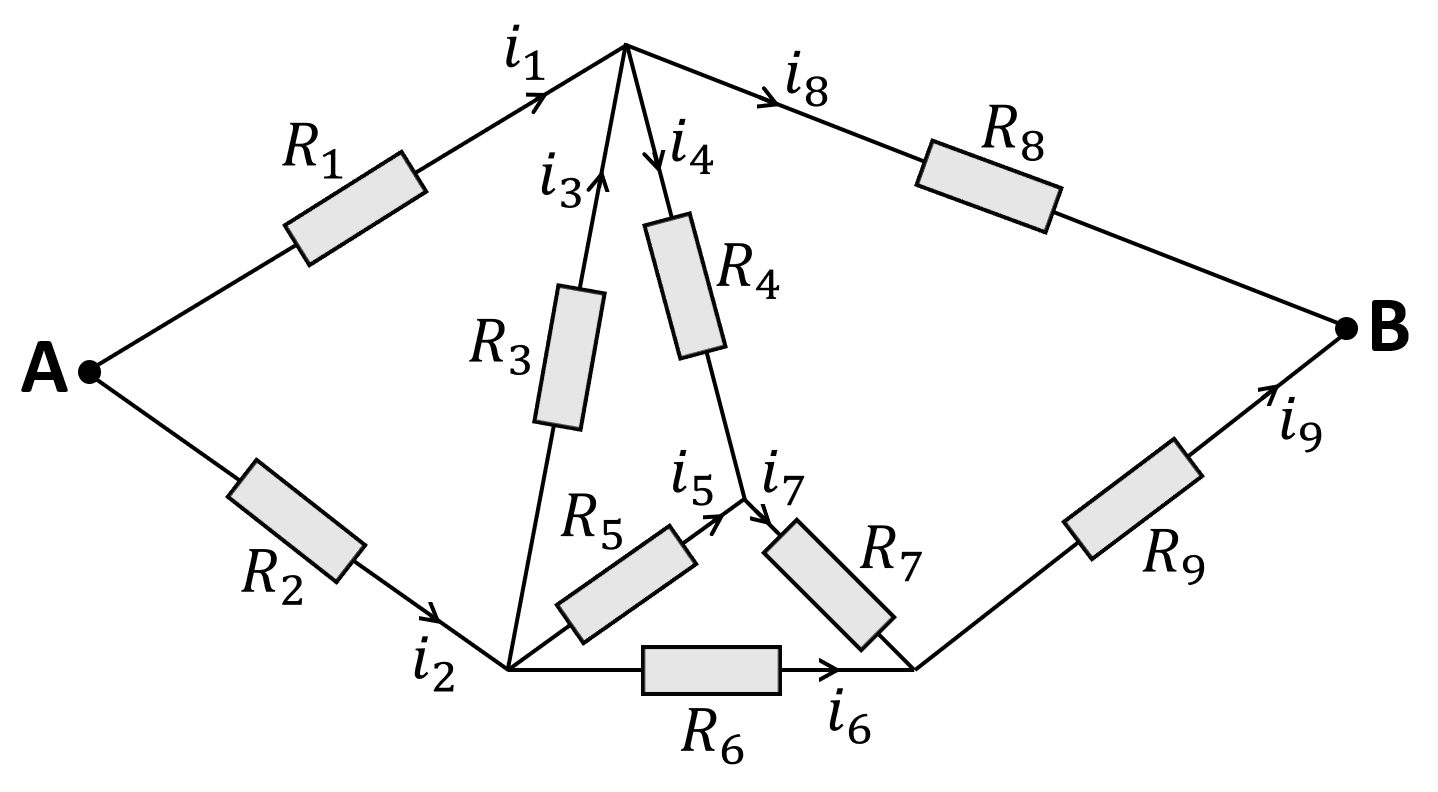
\includegraphics[width=0.6\textwidth,keepaspectratio]{Problem_2/Figs/P2A.png}
\end{figure}

Xét một mạch điện cấu tạo từ các điện trở $R_1$, $R_2$, ..., $R_8$, $R_9$. Khi đặt hiệu điện thế $1V$ vào hai đầu mạch A và B thì thu được phân bố dòng điện với chiều đi như hình vẽ, cường độ đo được theo đơn vị $mA$ là:
\begin{equation}
i_1 = 33 \ , \ i_2 = 28 \ , \ i_3 = 5 \ , \ i_4 = 2 \ , \ i_5 = 7 \ , \ i_6 = 16 \ , \ i_7 = 9 \ , \ i_8 = 36 \ , \ i_9 = 25 \ . \nonumber
\end{equation}
Với những thông tin đã cho thì liệu có thể xác định được giá trị của các điện trở hay không, và nếu có thì hãy xác định $R_1$ và $R_9$.

\newpage

{\normalcolor \textbf{CÂU 3}}\vspace{1.5mm}

\setcounter{equation}{0}
\textbf{Mạch chuyển đổi tín hiệu số - tương tự (DAC)}\footnote{ADC: Analog Digital Converter.}

Trong nhiều năm qua, công nghệ số (Digital) với các tín hiệu rời rạc được tổ hợp bởi các bit hai trạng thái 0 và 1\footnote{Trạng thái 0 ứng với dòng điện và điện áp ở mức "thấp" và trạng thái 1 ứng với dòng điện ở mức "cao" trong một chuẩn quy ước. Ví dụ với một số chip, trạng thái 0 ứng với điện áp \( \SI{0}{V} \), trạng thái 1 ứng với điện áp \( \SI{5}{V} \).}, đang dần thay thế các công nghệ tương tự (Analog) với tín hiệu là đại lượng vật lý có giá trị liên tục, trong việc truyền và xử lý, tính toán tín hiệu. Sự chuyển đổi công nghệ này là cần thiết và phù hợp để tín hiệu số ít bị ảnh hưởng bởi các nhiễu của môi trường tạo ra. Nhằm thực hiện các thao tác điều khiển ở đầu ra sau khi xử lý tín hiệu, chúng ta cần một bộ chuyển đổi từ tín hiệu số (dạng các số nhị phân tổ hợp bởi 0 và 1) sang tín hiệu tương tự (dạng các số tự nhiên liên tiếp). Ở bài toán này, chúng ta sẽ khảo sát các mô hình mạch DAC 4 bit đơn giản để hiểu được cơ chế của bộ chuyển đổi này.

%\includegraphics{Problem_3/DAC-Digital-to-Analog-Converter.png}
\begin{figure}[ht]
    \centering
        \scalebox{0.7}{
        

\tikzset{every picture/.style={line width=0.75pt}} %set default line width to 0.75pt        

\begin{tikzpicture}[x=0.75pt,y=0.75pt,yscale=-1,xscale=1]
%uncomment if require: \path (0,10708); %set diagram left start at 0, and has height of 10708

%Shape: Square [id:dp7634408012332572] 
\draw  [line width=1.5]  (448,9732) -- (498,9732) -- (498,9782) -- (448,9782) -- cycle ;
%Shape: Square [id:dp20939471942077437] 
\draw  [line width=1.5]  (448,9782) -- (498,9782) -- (498,9832) -- (448,9832) -- cycle ;
%Shape: Square [id:dp7345598092767369] 
\draw  [line width=1.5]  (448,9832) -- (498,9832) -- (498,9882) -- (448,9882) -- cycle ;
%Shape: Square [id:dp925543117058345] 
\draw  [line width=1.5]  (448,9882) -- (498,9882) -- (498,9932) -- (448,9932) -- cycle ;
%Shape: Square [id:dp39184346268946824] 
\draw  [line width=1.5]  (448,9932) -- (498,9932) -- (498,9982) -- (448,9982) -- cycle ;

%Straight Lines [id:da19312308479916473] 
\draw [line width=3]    (534,9858) -- (625.5,9858) ;
\draw [shift={(631.5,9858)}, rotate = 180] [fill={rgb, 255:red, 0; green, 0; blue, 0 }  ][line width=0.08]  [draw opacity=0] (16.97,-8.15) -- (0,0) -- (16.97,8.15) -- cycle    ;
%Shape: Rectangle [id:dp19162202320534494] 
\draw  [line width=2.25]  (664,9768) -- (769.5,9768) -- (769.5,9938) -- (664,9938) -- cycle ;

%Straight Lines [id:da16165597340033] 
\draw [line width=3]    (785.5,9857) -- (847.5,9857) ;
\draw [shift={(853.5,9857)}, rotate = 180] [fill={rgb, 255:red, 0; green, 0; blue, 0 }  ][line width=0.08]  [draw opacity=0] (16.97,-8.15) -- (0,0) -- (16.97,8.15) -- cycle    ;
%Straight Lines [id:da09877560081269832] 
\draw    (864,9930) -- (1068.5,9930) ;
%Straight Lines [id:da25437838858287787] 
\draw    (864,9930) -- (864,9757) ;
%Curve Lines [id:da07716136118610839] 
\draw [line width=2.25]    (864,9930) .. controls (908.5,9784) and (928.5,9751) .. (966.5,9821) ;
%Curve Lines [id:da7390366644901443] 
\draw [line width=2.25]    (966.5,9821) .. controls (987.5,9855) and (1026.5,9851) .. (1066.5,9821) ;

% Text Node
\draw (405,10004) node [anchor=north west][inner sep=0.75pt]   [align=left] {{\LARGE Tín hiệu số}};
% Text Node
\draw (857,10003) node [anchor=north west][inner sep=0.75pt]   [align=left] {{\LARGE Tín hiệu tương tự }};
% Text Node
\draw (716.63,9842) node [anchor=north] [inner sep=0.75pt]  [font=\small] [align=left] {{\fontfamily{pcr}\selectfont {\Huge DAC}}};
% Text Node
\draw (464,9941) node [anchor=north west][inner sep=0.75pt]   [align=left] {\textbf{{\fontfamily{pcr}\selectfont {\Large 0}}}};
% Text Node
\draw (464,9892) node [anchor=north west][inner sep=0.75pt]   [align=left] {{\fontfamily{pcr}\selectfont \textbf{{\Large 1}}}};
% Text Node
\draw (464,9840) node [anchor=north west][inner sep=0.75pt]   [align=left] {\textbf{{\fontfamily{pcr}\selectfont {\Large 0}}}};
% Text Node
\draw (464,9791) node [anchor=north west][inner sep=0.75pt]   [align=left] {{\fontfamily{pcr}\selectfont \textbf{{\Large 1}}}};
% Text Node
\draw (464,9741) node [anchor=north west][inner sep=0.75pt]   [align=left] {{\fontfamily{pcr}\selectfont \textbf{{\Large 1}}}};
\end{tikzpicture}
}
\caption{Sơ đồ biến đổi Digital - Analog}
\label{Sơ đồ biến đổi Digital - Analog }
\end{figure}
\begin{center}
\begin{enumerate}[label=(\alph*)]
    \item\textbf{Mạch khuếch đại đảo}
    
    Một linh kiện được sử dụng thường xuyên trong mạch chuyển đổi tín hiệu số là OPAMP (Operation amplifier). Xét mạch như hình sau, biết rằng ở trạng thái lý tưởng của mạch hiệu điện thế giữa hai điểm ở hai đầu $(+)$ và $(-)$ là bằng $0$ và không có dòng điện đi qua nhánh nối giữa $M$ và OPAMP. Đầu $(+)$ được nối với thành phần được gọi là nối đất\footnote{Dây nối đất sẽ coi như nối vào một nguồn có điện thế bằng 0. }. Biết rằng hai đại lượng $V_{out}$ và $V_{in}$ tỉ lệ với nhau qua một hằng số $\alpha$, cụ thể là $V_{out} = \alpha V_{in}$. Tìm $\alpha$ theo $R_0$ và $R_f$.
    \begin{figure}[H]
        \centering
        \scalebox{1}{  
        \begin{circuitikz}[european]
        { \sffamily <
        [american,font=\small]
        \draw
        (0,0) node[op amp] (opamp) {}
        (opamp.+) to [short] ++ (-0.0025,0) to ++(0,-1)
        (opamp.-) to ++(-1,0)
        to [short, -o] (-1.19,0.49) node[below]{$M$}
        (opamp.out) to [short,-*] ++(0.62,0) node[right] {}
        (1.75,-0.5) node[right]{$V_\text{out}$}
        (opamp.-) to [short] ++(0,1) to [R,l={$R_f$}] ++(2.4,0) to[short, -*] (opamp.out)
        (-2,0.49) to [R, l_=$R_0$] (-4,0.49)
        to [short, -o] (-5,0.49) node[left]
        {$V_\text{in}$}
        (-2,0.49) to [R, l_=$R_0$,i<=$I$] (-4,0.49)
        (-1.19,-1.5) -- (-1.19,-1) node[ground]{};
        > }
        ;\end{circuitikz}}
        \caption{Mạch khuếch đại đảo}
        \label{fig:60}
    \end{figure}        
    

    
    \item \textbf{Mạch DAC R/2nR (Binary Weighted Input DAC)}
    \begin{figure}[H]
          \centering
         \scalebox{1}{  
         \begin{circuitikz}[european]
         { \sffamily <
         [american,font=\small]
\draw 
(0,-0.7727) node[op amp] (opamp) {}
(opamp.+) to [short] ++ (-0.0025,0) to ++(0,-1.75) node[ground]{}
(opamp.-) to ++(-1.316,0)  %Phần dây cực âm kéo dài%
(opamp.out) to [short,-o] ++(0.62,0) node[right] {}
(1.75,-0.5) node[right]{$V_\text{out}$}{}
(opamp.-) to [short] (-1.19,1)  
(-1.19,1) to [R] (1.5,1)
(0.21,1.125) node[above]{$R_f$}
(1.5,1) to (1.5,-0.775)

(-1.19,-0.27) to [short, -o] (-1.19,-0.27) node[below]{$M$}
(-8, -0.28125) to  (-8, -4.03125)
;
\draw[ultra thick]
(-6.5,-0.28125) to (-5.75,-0.15125) node[above]{$K_0$} {}
(-6.5,-1.53125) to (-5.75,-1.40125) node[above]{$K_1$} {}
(-6.5,-2.78125) to (-5.75,-2.78125) node[above]{$K_2$} {}
(-6.5,-4.03125) to (-5.75,-3.87125) node[above]{$K_3$} {}
;
\draw 
(-8,-0.28125) to (-6.5, -0.28125)
(-6.5, -0.28125) to [short, -o] (-6.5,-0.28125)
(-8,-1.53125) to (-6.5, -1.53125)
(-6.5, -1.53125) to [short, -o] (-6.5,-1.53125)
(-8,-2.78125) to (-6.5, -2.78125)
(-6.5, -2.78125) to [short, -o] (-6.5,-2.78125)
(-8,-4.03125) to (-6.5, -4.03125)
(-6.5, -4.03125) to [short, -o] (-6.5,-4.03125)
(-8,-0.28125) node[above right]{$b_0 = 0$} {}
(-8,-1.53125) node[above right]{$b_1 = 0$} {}
(-8,-2.78125) node[above right]{$b_2 = 1$} {}
(-8,-4.03125) node[above right]{$b_3 = 0$} {}

(-2.5, -4.03125) to (-3.5, -4.03125)
(-2.5, -2.78125) to (-3.5, -2.78125)
(-2.5, -1.53125) to (-3.5, -1.53125)
(-2.5, -0.28125) to (-3.5, -0.28125)
(-3.5, -0.28125) to [R, l_=$2^0 R$] (-4.75, -0.28125)
(-3.5, -1.53125) to [R, l_=$2^1 R$] (-4.75, -1.53125)
(-3.5, -2.78125) to [R, l_=$2^2 R$] (-4.75, -2.78125)
(-3.5, -4.03125) to [R, l_=$2^3 R$] (-4.75, -4.03125)
(-4.75,-4.03125) to (-5.75,-4.03125)
(-4.75,-2.78125) to (-5.75,-2.78125)
(-4.75,-1.53125) to (-5.75,-1.53125)
(-4.75,-0.28125) to (-5.75,-0.28125)
(-5.75,-4.03125) to [short, -o] (-5.75,-4.03125)
(-5.75,-2.78125) to [short, -o] (-5.75,-2.78125)
(-5.75,-1.53125) to [short, -o] (-5.75,-1.53125)
(-5.75,-0.28125) to [short, -o] (-5.75,-0.28125)
(-2.5, -4.03125) to (-2.5, -0.28125)
(-9, -0.28125) to (-8, -0.28125)
(-9,-0.28125) to[short, -o]  (-9, -0.28125) node[left]{$V_\text{in}$} {}
(-2.5, -4.03125) to[short]  (-2.5, -4.03125) 
 ;
     > }
\end{circuitikz}}
%%Có thể cân nhắc nâng mạch này lên dạng tổng quát, tức là sẽ tăng lên thành vô hạn mắt mạch/thêm số lượng bit%%
         \caption{Mạch DAC R/2nR 4 Bit ở trạng thái 0010.}
         \label{fig:61}
    \end{figure}
   % Mạch chuyển đổi tín hiệu điện tử sang tín hiệu tương tự (DAC) là mạch chuyển đổi dãy các giá trị nhị phân (0100, 1000) thành giá trị tương tự. Xét trong trường hợp này, mạch 4 bit nghĩa là đang chuyển đổi giá trị từ dãy 4 giá trị nhị phân, với quy ước khi khóa $K_n$ nào đó mở (Nối đến đầu dương của OPAMP) là có giá trị nhị phân là 0 còn khi đóng (Nối đến đầu âm của OPAMP) là có giá trị 1. Để thể hiện thứ tự và mức độ quan trọng của giá trị nhị phân trong dãy, các điện trở được xếp theo thứ tự từ phải sang trái và tăng dần theo cấp số nhân cũng như về mức độ quan trọng. (Ở điện trở $2^0 R$ tương ứng với giá trị nhị phân $b_0$ thì $b_0$ là giá trị nhị phân quan trọng nhất và tương tự thì $b_3$ là giá trị nhị phân kém quan trọng nhất, tương ứng với điện trở %2^3 R$.

   Trong phần này, ta sẽ xét một mạch thể hiện được $4$ bit thông tin (hay $4$ giá trị nhị phân) như hình (\ref{fig:61}). Quy ước về các giá trị nhị phân là: khi khoá $K_n$ mở thì tương đương với giá trị nhị phân $0$; khi khoá $K_n$ đóng thì tương đương giá trị nhị phân $1$. Với $n$ tương ứng với số mũ của điện trở ($2^n R$) mà khoá $K$ mắc nối tiếp. Các trạng thái này được biểu diễn qua các giá trị $b_n$ được ghi trên hình.

   Khi thể hiện dãy thông tin $4$ bit, ta sẽ ghi nhận trạng thái của các khoá $K$. Với thứ tự lần lượt từ trái sang phải là từ $n=0$ đến $n=3$.
   
    Cho các giá trị $V_{in}$, $R$ và $R_f$ coi như đã biết. Hãy tính giá trị của điện thế $V_{out}$ dựa theo các giá trị trên và tương ứng với các tín hiệu nhị phân 4 bit trong bảng \ref{Bảng chuyển đổi tín hiệu(Đề bài)}. Để có một bảng giá trị đẹp mắt, ta chọn đơn vị của $V_{out}$ là $\left( -\frac{R_f}{8R}V_{in}\right)$.
    \begin{table}[ht]
    \hspace{0.15\textwidth}
    \begin{tabular}{|c|c|c|c|c|c|c|c|c|}
    \hline
    Tín hiệu số & 0000 & 0001 & 0010 & 0011 & 0100 & 0101 & 0110 & 0111 \\ \hline
    $V_{out} $  &      &      &      &      &      &      &      &      \\ \hline
    
    \end{tabular}
    \end{table}

    \begin{table}[ht]
    \hspace{0.15\textwidth}
    \begin{tabular}{|c|c|c|c|c|c|c|c|c|}
    \hline
    Tín hiệu số & 1000 & 1001 & 1010 & 1011 & 1100 & 1101 & 1110 & 1111 \\ \hline
    $V_{out} $  &      &      &      &      &      &      &      &      \\ \hline

    \end{tabular}
    \caption{}
    \label{Bảng chuyển đổi tín hiệu(Đề bài)}
    \end{table}
    \item \textbf{Mạch DAC R-2R (Ladder DAC)}
    
    Có thể nhận thấy, nhược điểm lớn nhất của mạch DAC dạng R/2nR là việc sử dụng quá nhiều điện trở chính xác để thực hiện quá trình chuyển đổi và khi mà các số bit đầu vào tăng lên thì giá trị điện trở sẽ tăng lên theo cấp số nhân. Vì vậy, một biến thể được sử dụng rộng rãi hơn là dạng R-2R vốn chỉ sử dụng tới 2 loại điện trở. Mạch điện ấy có dạng như sau:
    \begin{figure}[H]
         \centering
         \scalebox{1}{  
         \begin{circuitikz}[european]
         { \sffamily <
         [american,font=\small]
\draw 

(0,-0.7727) node[op amp] (opamp) {}
(opamp.+) to [short] ++ (-0.0025,0) to ++(0,-1.75) node[ground]{}
(opamp.-) to ++(-1.316,0)  %Phần dây cực âm kéo dài%
(opamp.out) to [short,-o] ++(0.62,0) node[right] {}
(1.75,-0.5) node[right]{$V_\text{out}$}{}
(opamp.-) to [short] (-1.19,1)  
(-1.19,1) to [R] (1.5,1)
(0.21,1.125) node[above]{$R_f$}
(1.5,1) to (1.5,-0.775)

(-1.19,-0.27) to [short, -o] (-1.19,-0.27) node[below]{$M$}

(-1.19, -0.2825) to (-3.5, -0.2825)
(-3.5, -0.2825) to (-3.5, -0.7825)
(-3.5, -0.7825) to [R, l_=$2R$] (-3.5, -2.2825)
(-3.5, -2.2825) to (-3.5,-2.5)
;
\draw[ultra thick]
(-3.5,-2.5) to (-3, -3)
(-5,-2.5) to (-4.5, -3) 
(-6.5, -2.5) to (-6.5, -3)
(-8,-2.5) to (-7.5, -3)
;
\draw
(-3.5, -3) to (-3.5, -4.25)
(-5, -3) to (-5, -4.25)
(-6.5, -3) to (-6.5, -4.25)
(-8, -3) to (-8, -4.2525)

(-3.5, -0.2825) to [R, l_=$R$] (-5, -0.2825)
(-5, -0.2825) to (-5, -0.7825)
(-5, -0.7825) to [R, l_=$2R$] (-5, -2.2825)
(-5, -2.2825) to (-5,-2.5)

(-5, -0.2825) to [R, l_=$R$] (-6.5, -0.2825)
(-6.5, -0.2825) to (-6.5, -0.7825)
(-6.5, -0.7825) to [R, l_=$2R$] (-6.5, -2.2825)
(-6.5, -2.2825) to (-6.5,-2.5)

(-6.5, -0.2825) to [R, l_=$R$] (-8, -0.2825) node[above]{}
(-8, -0.2825) to (-8, -0.7825)
(-8, -0.7825) to [R, l_=$2R$] (-8, -2.2825)
(-8, -2.2825) to (-8,-2.5)

(-7.5, -3)node[ground]{}
(-6, -3)node[ground]{}
(-4.5, -3)node[ground]{}
(-3, -3)node[ground]{}
(-7.5, -3) to [short, -o] (-7.5, -3)
(-6, -3) to [short, -o] (-6, -3)
(-4.5, -3) to [short, -o] (-4.5, -3)
(-3, -3) to [short, -o] (-3, -3)

(-7, -2.75)node[left]{$K_3$}
(-5.5, -2.75)node[left]{$K_2$}
(-4, -2.75)node[left]{$K_1$}
(-2.5, -2.75)node[left]{$K_0$}

(-6.75, -3.9)node[left]{$b_3=0$}
(-5.25, -3.9)node[left]{$b_2=1$}
(-3.75, -3.9)node[left]{$b_1=0$}
(-2.25, -3.9)node[left]{$b_0=0$}

(-3.5, -4.25) to (-9, -4.25)
(-9, -4.25) to [short, -o] (-9, -4.25) node[left]{$V_\text{in}$} {}

(-8, -0.2825) to (-9.5, -0.2825)
(-9.5, -0.2825) to (-9.5, -0.7825)
(-9.5, -0.7825) to [R, l_=$2R$] (-9.5,  -2.2825)
(-9.5,  -2.2825) to (-9.5,  -3)node[ground]{}

(-3.5, -3) to [short, -o] (-3.5, -3)
(-5, -3) to [short, -o] (-5, -3)
(-6.5, -3) to [short, -o] (-6.5, -3)
(-8, -3) to [short, -o] (-8, -3)

(-3.5,-2.5) to [short, -o] (-3.5,-2.5)
(-5,-2.5) to [short, -o] (-5,-2.5) 
(-6.5,-2.5) to [short, -o] (-6.5,-2.5) 
(-8,-2.5) to [short, -o] (-8,-2.5)
 ;
  \draw[dashed]
 (-2,1) to (-10.5,1)
 (-10.5,1) to (-10.5,-5)
 (-10.5,-5) to (-2,-5)
 (-2,-5) to (-2,1)
 ;
 >}
\end{circuitikz}}
        \caption{Mạch DAC R-2R 4 Bit ở trạng thái 0010}
        \label{fig:64}
    \end{figure} 
    \begin{figure}[H]
        \centering
        \begin{circuitikz}[european]
\draw
(0,-0.7727) node[op amp] (opamp) {}
(opamp.+) to [short] ++ (-0.0025,0) to ++(0,-1) node[ground]{}
(opamp.-) to ++(-1.316,0)  %Phần dây cực âm kéo dài%
(opamp.out) to [short,-o] ++(0.62,0) node[right] {}
(1.75,-0.5) node[right]{$V_\text{out}$}{}
(opamp.-) to [short] (-1.19,1)  
(-1.19,1) to [R] (1.5,1)
(0.21,1.125) node[above]{$R_f$}
(1.5,1) to (1.5,-0.775)

(-1.19,-0.27) to [short, -o] (-1.19,-0.27)  node[below]{$M$}
(-1.19,-0.2825) to (-3,-0.2825)
(-3,-0.2825) to [R, l_=$R_0$] (-5,-0.2825)
(-5,-0.2825) to (-5,-2)
(-5,-2) to [short, -o] (-5,-2) node[left]
{$V_\text{R-2R}$}
;
\draw [dashed]
(-2,1) to (-2,-3)
(-2,-3) to (-6.5,-3) 
%(-4.25,-3)node[below]{Hệ tương đương}
(-6.5,-3) to (-6.5, 1)
(-6.5, 1) to (-2,1)
;
\end{circuitikz}
        \caption{Hệ tương đương của mạch R-2R}
        \label{fig:65}
    \end{figure}
%Hãy đi khảo sát giá trị của $V_{out}$ tại những trạng thái $0001$, $0010$, $0100$ và $1000$. Từ đấy, sử dụng nguyên lý chồng chập để tìm ra quy luật chung của $V_{out}$ dựa theo các trạng thái của khoá $K$. Nguyên lý chồng chập có thể hiểu là: "trong một mạch điện tuyến tính có nhiều nguồn độc lập, tổng ảnh hưởng của các nguồn sẽ bằng tổng đại số các ảnh hưởng của từng nguồn". 

Hệ mạch điện nằm trong khung sẽ tương đương với một điện thế $V_{R-2R}$ và một điện trở $R_0$ như hình (\ref{fig:65}). Các giá trị điện thế và điện trở có thể bị thay đổi bởi trạng thái của khoá $K$.
\begin{enumerate}
    \item[1.] Khi mạch điện ở trạng thái $0000$, tìm $V_{R-2R}$ và $R_0$.
    \item[2.] Khi mạch điện ở trạng thái $0001$ và $1000$, tìm $V_{R-2R}$ và $R_0$. 
    \item[3.] Sử dụng tính tương tự để tính $V_{R-2R}$ và $R_0$ cho mạch ở trạng thái $0100$ và $0010$.
    \item[4.] Sử dụng nguyên lý chồng chập để đưa ra quy luật chung cho điện thế $V_{out}$ theo các giá trị $b_n, R, R_f$ và $V_{in}$. Nguyên lý chồng chập phát biểu: "\textit{Ảnh hưởng do các nguồn độc lập gây ra, bằng tổng ảnh hưởng của từng nguồn gây ra}".
\end{enumerate}
%Các dây nối đất là những dây nối vào một nguồn có điện thế bằng $0$. Vì thế, ta có thể coi như có dây dẫn giữa các đầu nối đất trong mạch.  

Gợi ý: Sử dụng định lý Thevenin.
\end{enumerate}
\end{center}
\begin{flushright}
   \normalcolor(Biên soạn bởi Mino và trees\&streetslights.inc)
\end{flushright}

\newpage

{\normalcolor \textbf{CÂU 4}}\vspace{1.5mm}

\setcounter{equation}{0}
\textbf{Thấu kính tứ cực từ hội tụ mạnh}

Trong các máy gia tốc hạt năng lượng cao, việc điều hướng chuyển động của các hạt cần thông qua các tương tác điện từ. Tứ cực từ là một mô hình từ trường tạo ra bởi hệ thống dây điện được cuốn để sinh ra từ trường có dạng đường sức khá giống với bốn nam châm đặt đối xứng bốn góc và thường được sử dụng cho mục đích điều hướng chùm hạt. Trường điện từ của tứ cực từ sẽ tác dụng lực lên các hạt khiến cho quỹ đạo của chúng bị bẻ cong như cách các tia sáng đi qua các thấu kính quang học, nhưng lại chỉ bẻ hướng tia sáng về phía quang trục (như thấu kính hội tụ) theo một phương và bẻ hướng tia sáng ra xa khỏi quang trục (như thấu kính phân kỳ) theo phương còn lại. Trong bài toán này, chúng ta sẽ khảo sát định tính về mô hình tứ cực từ cũng như thiết kế một hệ các thấu kính tứ cực để tạo ra sự hội tụ cho chùm hạt.


\begin{enumerate}
    \item \textbf{Tính chất thú vị của tứ cực từ} \\
    Khi bạn lắp ráp bốn nam châm điện lại thành một hệ sao cho hai cực Nam ở đối diện nhau và hai cực Bắc ở đối diện nhau như hình \ref{fig:41}, bạn sẽ thu được một \textbf{tứ cực từ}. Tứ cực từ có rất nhiều tính chất thú vị, và được sử dụng rộng rãi trong các máy gia tốc hạt nhằm hội tụ các chùm tia tích điện. Các câu hỏi phía dưới sẽ khảo sát các đặc tính độc đáo của tứ cực từ:
    
    \begin{center}
    \begin{minipage}{0.45\textwidth}
    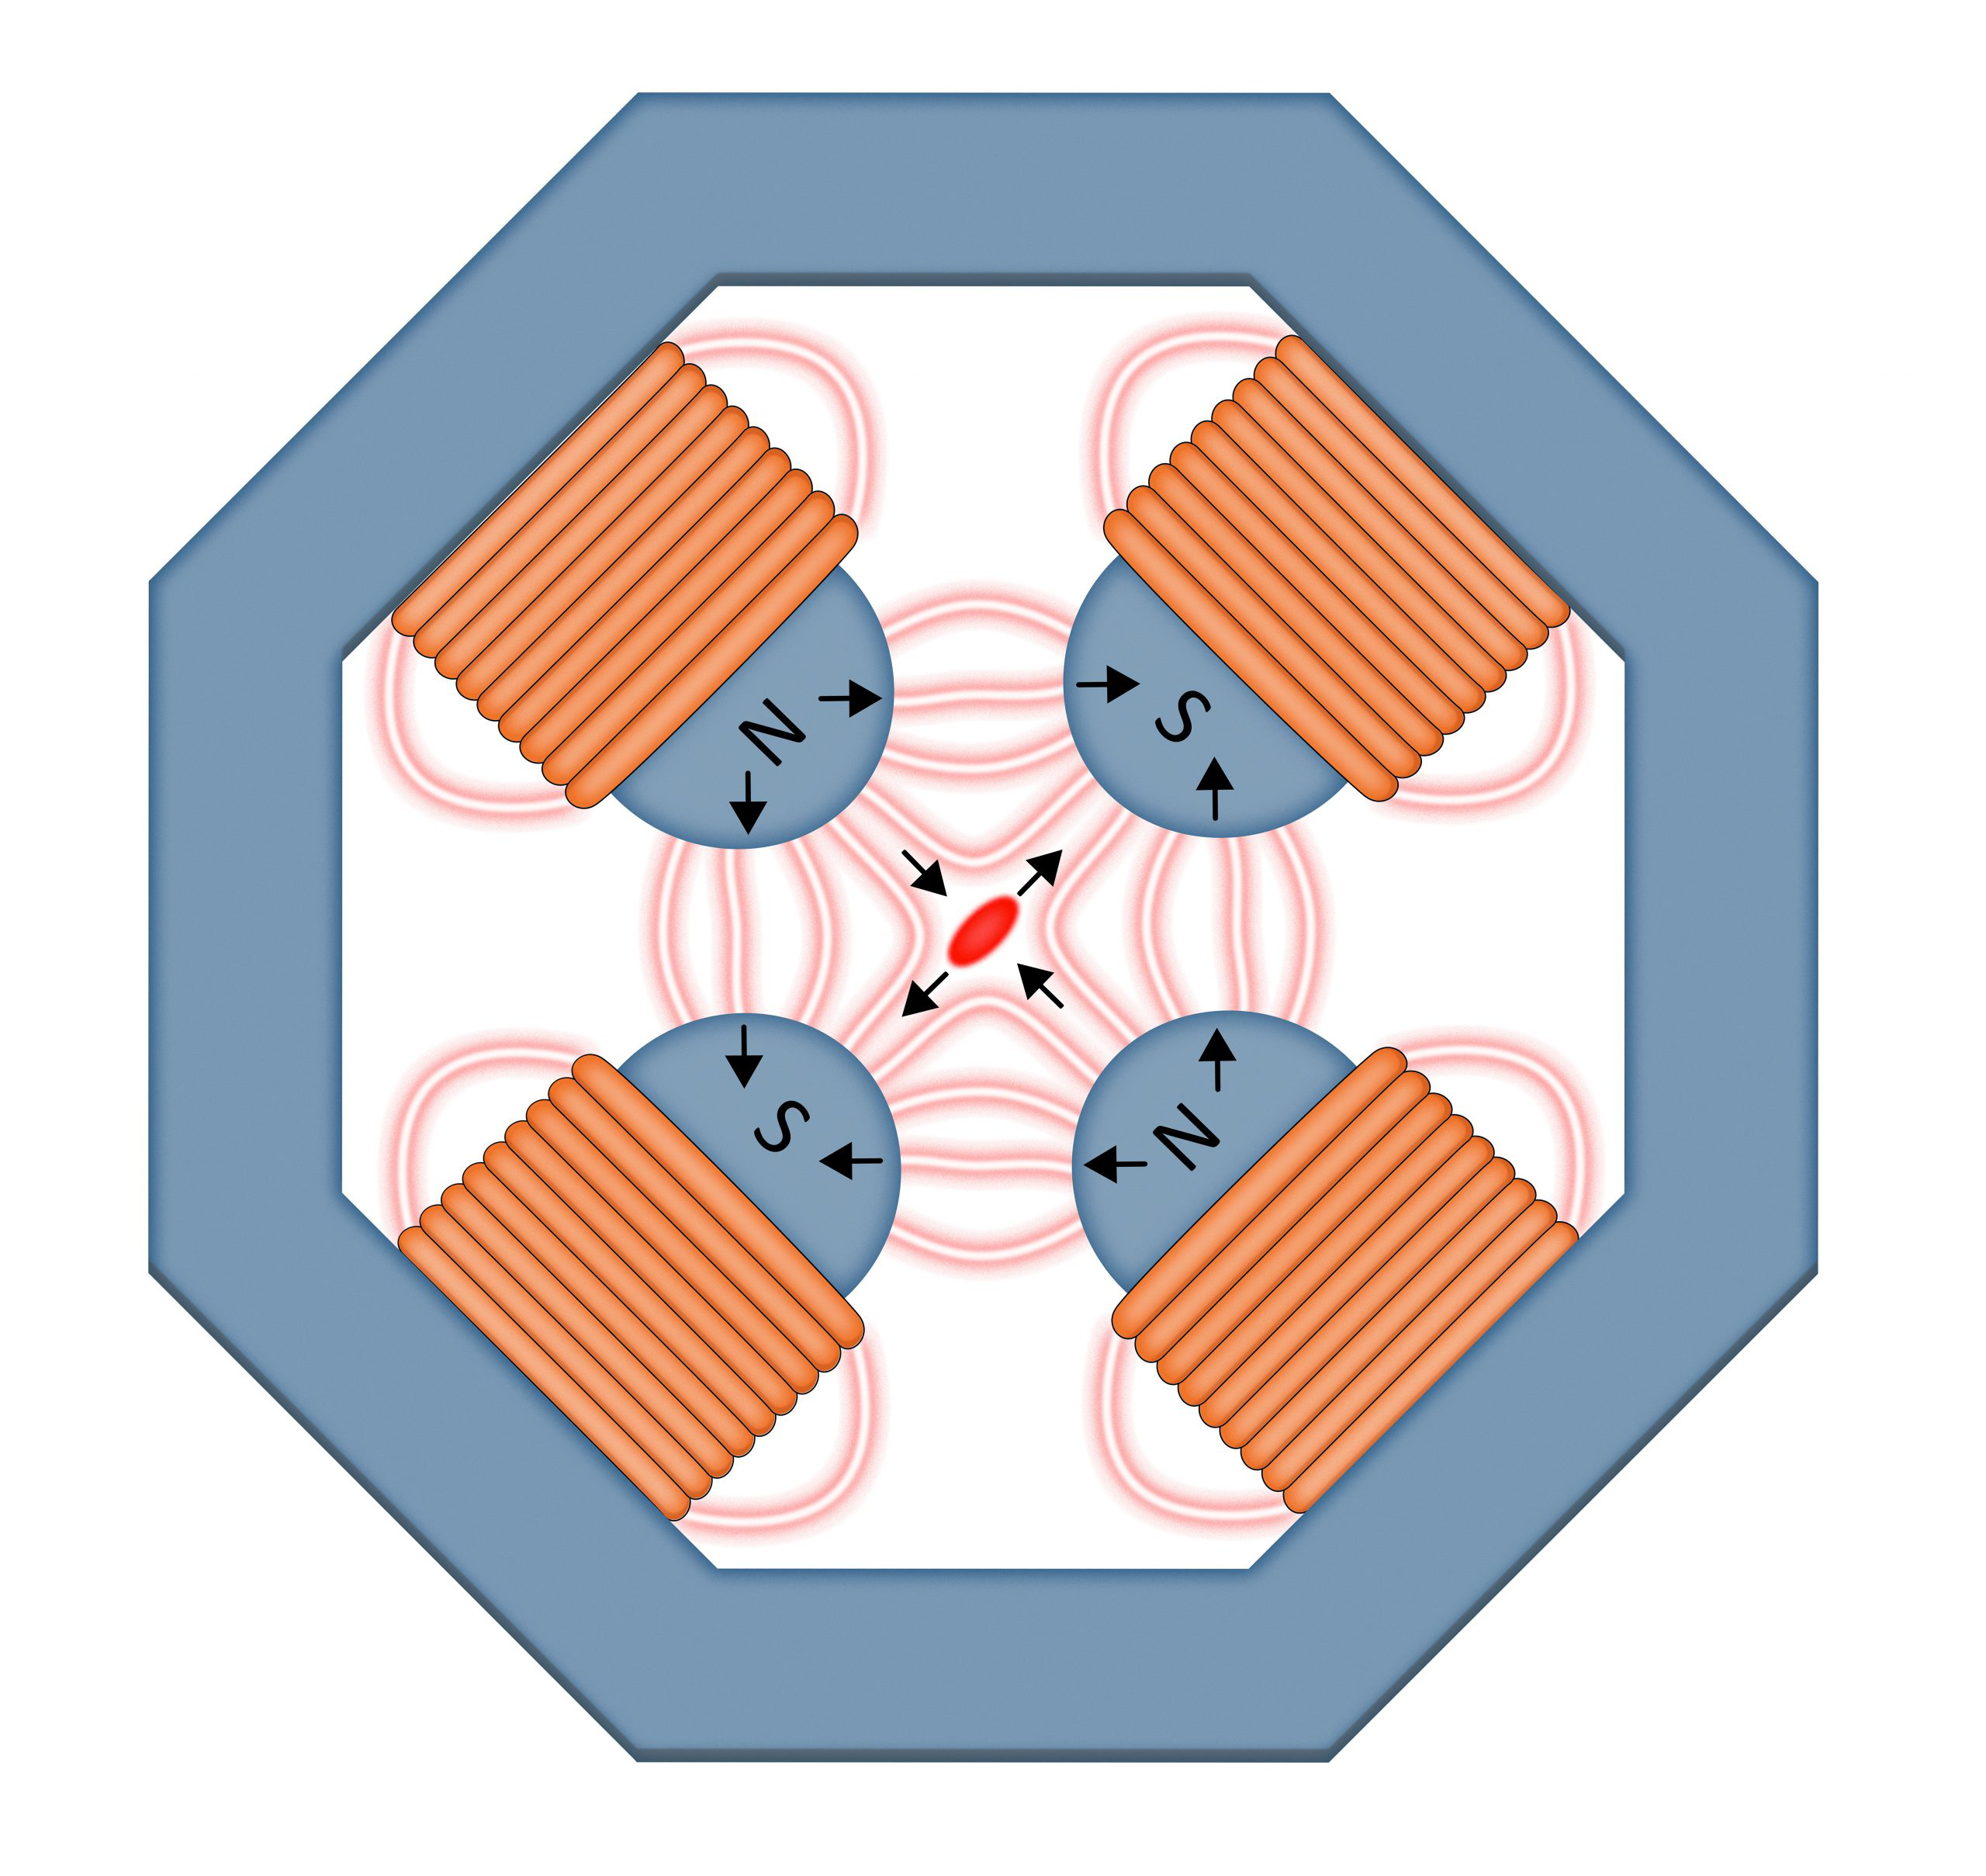
\includegraphics[width=0.9\textwidth]{Problem_4/quadrupoles.png}
    \end{minipage}
    \begin{minipage}{0.45\textwidth}
    \centering
    \scalebox{0.5}{
    \begin{tikzpicture}[x=0.75pt,y=0.75pt,yscale=-1,xscale=1]
        %uncomment if require: \path (0,642); %set diagram left start at 0, and has height of 642
        
        %Curve Lines [id:da4792522475831378] 
        \draw    (266,156) .. controls (356,227) and (358,227) .. (444,155) ;
        %Curve Lines [id:da18776678628173316] 
        \draw    (257,165) .. controls (365,254) and (349,254) .. (454,164) ;
        %Curve Lines [id:da7579049508332776] 
        \draw    (249,173) .. controls (367,283) and (346,283) .. (463,174) ;
        %Curve Lines [id:da9068961265681277] 
        \draw    (276,146) .. controls (354,204) and (363,204) .. (432,144) ;
        %Curve Lines [id:da6057096352515956] 
        \draw    (287,136) .. controls (356,191) and (359,191) .. (421,132) ;
        %Curve Lines [id:da6124834939512256] 
        \draw    (298,126) .. controls (346,161) and (367,161) .. (410,122) ;
        %Curve Lines [id:da999176140900975] 
        \draw    (309,115) .. controls (345,144) and (371,145) .. (403,114) ;
        %Curve Lines [id:da4412765595880592] 
        \draw    (315,108) .. controls (340,122) and (375,121) .. (397,108) ;
        %Curve Lines [id:da6165862171426286] 
        \draw    (327,97) .. controls (349,108) and (367,107) .. (386,97) ;
        %Curve Lines [id:da5352330674257251] 
        \draw    (337,86) .. controls (353,93) and (361,93) .. (373,85) ;
        %Straight Lines [id:da13696112022895202] 
        \draw    (241.18,179.89) -- (469.82,407.11) ;
        %Straight Lines [id:da612929119766775] 
        \draw    (239.67,405.57) -- (471.33,181.43) ;
        %Curve Lines [id:da9013347475427187] 
        \draw    (209.43,380.62) .. controls (281.45,292.07) and (284.48,289.13) .. (212.07,202.64) ;
        %Curve Lines [id:da8829915710419369] 
        \draw    (218.14,389.8) .. controls (308.32,283.62) and (308,299.62) .. (221.17,192.82) ;
        %Curve Lines [id:da839350917569065] 
        \draw    (225.88,397.96) .. controls (335.11,279.16) and (336.6,303.2) .. (231.24,184.02) ;
        %Curve Lines [id:da09708382750689237] 
        \draw    (199.74,370.42) .. controls (258.67,293.61) and (259.88,282.63) .. (200.95,214.41) ;
        %Curve Lines [id:da6233083389607426] 
        \draw    (190.08,359.22) .. controls (245.86,291.35) and (238.14,282.19) .. (188.87,225.17) ;
        %Curve Lines [id:da9303172125407404] 
        \draw    (180.42,348.02) .. controls (216,300.74) and (217.5,275.76) .. (178.76,235.96) ;
        %Curve Lines [id:da2769813795168756] 
        \draw    (169.77,336.8) .. controls (197.44,289.36) and (198.47,287.38) .. (170.71,242.8) ;
        %Curve Lines [id:da812357712173224] 
        \draw    (162.98,330.66) .. controls (176.4,302.93) and (177.05,270.94) .. (164.65,248.68) ;
        %Curve Lines [id:da730462575275286] 
        \draw    (152.35,318.44) .. controls (163.73,293.67) and (163.05,278.65) .. (153.55,259.45) ;
        %Curve Lines [id:da735579584390504] 
        \draw    (141.68,308.22) .. controls (148.93,292.37) and (147.11,284.33) .. (141.43,272.21) ;
        
        %Curve Lines [id:da9957314369504402] 
        \draw    (447.23,429.41) .. controls (356.24,360.51) and (353.19,357.59) .. (269.26,432.95) ;
        %Curve Lines [id:da42061516499279983] 
        \draw    (456.1,420.39) .. controls (346.85,333.94) and (362.85,333.72) .. (259.14,424.19) ;
        %Curve Lines [id:da6302289013179545] 
        \draw    (463.99,412.36) .. controls (341.47,307.32) and (365.44,305) .. (250,414.44) ;
        %Curve Lines [id:da6314722799353274] 
        \draw    (437.37,439.44) .. controls (358.56,383.22) and (347.55,382.39) .. (281.42,443.65) ;
        %Curve Lines [id:da7627601342878407] 
        \draw    (426.52,449.49) .. controls (356.74,396.1) and (347.86,404.14) .. (292.59,455.36) ;
        %Curve Lines [id:da5517437382717942] 
        \draw    (415.66,459.53) .. controls (367.17,425.61) and (342.16,424.98) .. (303.73,465.09) ;
        %Curve Lines [id:da2523109982366758] 
        \draw    (404.82,470.56) .. controls (356.44,444.56) and (354.42,443.6) .. (310.84,472.9) ;
        %Curve Lines [id:da5531448424788401] 
        \draw    (398.92,477.57) .. controls (370.73,465.12) and (338.74,465.57) .. (316.92,478.74) ;
        %Curve Lines [id:da8274878407169837] 
        \draw    (387.07,488.61) .. controls (361.92,478.1) and (346.93,479.3) .. (328.08,489.46) ;
        %Curve Lines [id:da2516778847803036] 
        \draw    (377.23,499.63) .. controls (361.13,492.94) and (353.16,495.03) .. (341.25,501.14) ;
        
        %Curve Lines [id:da44567985870338966] 
        \draw    (497.97,200.1) .. controls (426.63,289.2) and (423.63,292.16) .. (496.69,378.1) ;
        %Curve Lines [id:da18107514459279583] 
        \draw    (489.19,190.99) .. controls (399.82,297.86) and (400.03,281.86) .. (487.67,387.99) ;
        %Curve Lines [id:da3520275384011575] 
        \draw    (481.38,182.89) .. controls (373.06,302.52) and (371.39,278.5) .. (477.67,396.86) ;
        %Curve Lines [id:da5409134618202889] 
        \draw    (507.73,210.23) .. controls (449.39,287.49) and (448.27,298.48) .. (507.72,366.24) ;
        %Curve Lines [id:da5658457580650191] 
        \draw    (517.48,221.35) .. controls (462.22,289.65) and (470.02,298.75) .. (519.72,355.39) ;
        %Curve Lines [id:da41437201980134053] 
        \draw    (527.22,232.48) .. controls (492.01,280.03) and (490.7,305.02) .. (529.75,344.52) ;
        %Curve Lines [id:da607470080861005] 
        \draw    (537.96,243.62) .. controls (510.65,291.27) and (509.64,293.26) .. (537.75,337.62) ;
        %Curve Lines [id:da3226182027720166] 
        \draw    (544.8,249.7) .. controls (531.59,277.54) and (531.18,309.53) .. (543.76,331.7) ;
        %Curve Lines [id:da59845594322587] 
        \draw    (555.52,261.84) .. controls (544.33,286.7) and (545.13,301.71) .. (554.77,320.84) ;
        %Curve Lines [id:da3781492316292461] 
        \draw    (566.27,271.98) .. controls (559.15,287.89) and (561.02,295.91) .. (566.8,307.99) ;
        
        %Straight Lines [id:da8548346448041899] 
        \draw    (76,556) -- (74.01,44) ;
        \draw [shift={(74,42)}, rotate = 89.78] [color={rgb, 255:red, 0; green, 0; blue, 0 }  ][line width=0.75]    (10.93,-3.29) .. controls (6.95,-1.4) and (3.31,-0.3) .. (0,0) .. controls (3.31,0.3) and (6.95,1.4) .. (10.93,3.29)   ;
        %Straight Lines [id:da8984436400560898] 
        \draw    (76,556) -- (626,555) ;
        \draw [shift={(628,555)}, rotate = 179.9] [color={rgb, 255:red, 0; green, 0; blue, 0 }  ][line width=0.75]    (10.93,-3.29) .. controls (6.95,-1.4) and (3.31,-0.3) .. (0,0) .. controls (3.31,0.3) and (6.95,1.4) .. (10.93,3.29)   ;
        \draw   (349,222) -- (364,231) -- (349,240) ;
        \draw   (295.58,280.6) -- (286.41,295.5) -- (277.59,280.4) ;
        \draw   (365.2,365.83) -- (350,357.16) -- (364.8,347.84) ;
        \draw   (414.6,297.62) -- (423.4,282.5) -- (432.6,297.38) ;
        
        % Text Node
        \draw (183,119.4) node [anchor=north west][inner sep=0.75pt]  [font=\Huge,color={rgb, 255:red, 208; green, 2; blue, 27 }  ,opacity=1 ]  {$N$};
        % Text Node
        \draw (490,407.4) node [anchor=north west][inner sep=0.75pt]  [font=\Huge,color={rgb, 255:red, 208; green, 2; blue, 27 }  ,opacity=1 ]  {$N$};
        % Text Node
        \draw (503,120.4) node [anchor=north west][inner sep=0.75pt]  [font=\Huge,color={rgb, 255:red, 65; green, 117; blue, 5 }  ,opacity=1 ]  {$S$};
        % Text Node
        \draw (190,410.4) node [anchor=north west][inner sep=0.75pt]  [font=\Huge,color={rgb, 255:red, 65; green, 117; blue, 5 }  ,opacity=1 ]  {$S$};
        % Text Node
        \draw (42,559.4) node [anchor=north west][inner sep=0.75pt]  [font=\huge]  {$O$};
        % Text Node
        \draw (603,563) node [anchor=north west][inner sep=0.75pt]  [font=\huge]  {$x$};
        % Text Node
        \draw (42,34.4) node [anchor=north west][inner sep=0.75pt]  [font=\huge]  {$y$};


    \end{tikzpicture}
    }
    \end{minipage} \\
    %\caption{Mô hình tứ cực từ trong thực tế (bên trái) và từ phổ của tứ cực từ (bên phải)}
    \captionof{figure}{Mô hình tứ cực từ trong thực tế (bên trái) và từ phổ của tứ cực từ (bên phải)}
    \label{fig:41}
    \end{center}
    
    Cho từ phổ của một tứ cực từ. Dựa vào hình \ref{fig:41}, hãy xác định phương, chiều của \textbf{đường sức từ} và \textbf{lực điện từ} tác dụng lên một hạt điện tích nhỏ bay vào tứ cực từ với phương vuông góc với trang giấy, chiều ra xa người đọc. 

    \item \textbf{Ứng dụng trong việc hội tụ chùm tia} \\
    Sau khi đã xác định được lực điện từ tác dụng lên hạt điện tích, ta có thể thấy rằng theo phương $y$, hạt sẽ bị đẩy vào bên trong tứ cực từ, còn theo phương $x$, hạt sẽ bị đẩy ra xa tứ cực từ. Hay nói cách khác, nếu ta coi tứ cực từ là một thấu kính thì thấu kính này sẽ \textbf{hội tụ} trên phương $y$ và \textbf{phân kì} trên phương $x$ với cùng một tiêu cự $f$. Nếu ta lật ngược thấu kính đi $90^\circ$ thì thấu kính sẽ phân kỳ trên phương $y$ và hội tụ trên phương $x$.
    
    \begin{figure}[!ht]
    \centering
    \scalebox{0.9}{
    \begin{tikzpicture}[x=0.75pt,y=0.75pt,yscale=-1,xscale=1]
        %uncomment if require: \path (0,424); %set diagram left start at 0, and has height of 424
        
        %Straight Lines [id:da6678677431158608] 
        \draw    (51,378) -- (181,378) ;
        %Straight Lines [id:da673747824550079] 
        \draw    (51,259) -- (181,259) ;
        %Straight Lines [id:da3567165573223894] 
        \draw    (51,259) -- (51,378) ;
        %Straight Lines [id:da4131289268440297] 
        \draw    (181,259) -- (181,378) ;
        %Curve Lines [id:da6284585681017343] 
        \draw    (51,289) .. controls (82,288) and (82,284) .. (83,259) ;
        %Curve Lines [id:da7073873859904605] 
        \draw    (51,346) .. controls (83,348) and (83,348) .. (83,378) ;
        %Curve Lines [id:da3036947661512792] 
        \draw    (149,259) .. controls (150,291) and (150,291) .. (181,291) ;
        %Curve Lines [id:da9150242892043405] 
        \draw    (151,378) .. controls (151,346) and (151,346) .. (182,346) ;
        
        %Straight Lines [id:da8908202829099343] 
        \draw    (245,271) -- (375,271) ;
        %Straight Lines [id:da2173944797906926] 
        \draw    (245,152) -- (375,152) ;
        %Straight Lines [id:da3230976467548934] 
        \draw    (245,152) -- (245,271) ;
        %Straight Lines [id:da37549197915656185] 
        \draw    (375,152) -- (375,271) ;
        %Curve Lines [id:da11844780145514733] 
        \draw    (245,182) .. controls (276,181) and (276,177) .. (277,152) ;
        %Curve Lines [id:da19840673204511416] 
        \draw    (245,239) .. controls (277,241) and (277,241) .. (277,271) ;
        %Curve Lines [id:da07608929271157883] 
        \draw    (343,152) .. controls (344,184) and (344,184) .. (375,184) ;
        %Curve Lines [id:da590005125259021] 
        \draw    (345,271) .. controls (345,239) and (345,239) .. (376,239) ;
        %Straight Lines [id:da8314279294962961] 
        \draw  [dash pattern={on 0.84pt off 2.51pt}]  (181,378) -- (573,162) ;
        %Straight Lines [id:da09601563855642858] 
        \draw    (115,320) -- (205,320) ;
        \draw [shift={(207,320)}, rotate = 180] [color={rgb, 255:red, 0; green, 0; blue, 0 }  ][line width=0.75]    (10.93,-3.29) .. controls (6.95,-1.4) and (3.31,-0.3) .. (0,0) .. controls (3.31,0.3) and (6.95,1.4) .. (10.93,3.29)   ;
        %Straight Lines [id:da8517185652543424] 
        \draw    (115,320) -- (115,228) ;
        \draw [shift={(115,226)}, rotate = 90] [color={rgb, 255:red, 0; green, 0; blue, 0 }  ][line width=0.75]    (10.93,-3.29) .. controls (6.95,-1.4) and (3.31,-0.3) .. (0,0) .. controls (3.31,0.3) and (6.95,1.4) .. (10.93,3.29)   ;
        %Straight Lines [id:da9476216664675472] 
        \draw  [dash pattern={on 4.5pt off 4.5pt}]  (443,162) -- (573,162) ;
        %Straight Lines [id:da7668565905633495] 
        \draw  [dash pattern={on 4.5pt off 4.5pt}]  (443,43) -- (573,43) ;
        %Straight Lines [id:da6517531350813479] 
        \draw  [dash pattern={on 4.5pt off 4.5pt}]  (443,43) -- (443,162) ;
        %Straight Lines [id:da05757003100942071] 
        \draw  [dash pattern={on 4.5pt off 4.5pt}]  (573,43) -- (573,162) ;
        %Straight Lines [id:da1731975813788058] 
        \draw  [dash pattern={on 4.5pt off 4.5pt}]  (38,363) -- (600.25,51.97) ;
        \draw [shift={(602,51)}, rotate = 151.05] [color={rgb, 255:red, 0; green, 0; blue, 0 }  ][line width=0.75]    (10.93,-3.29) .. controls (6.95,-1.4) and (3.31,-0.3) .. (0,0) .. controls (3.31,0.3) and (6.95,1.4) .. (10.93,3.29)   ;
        %Shape: Circle [id:dp49351180655100846] 
        \draw  [fill={rgb, 255:red, 74; green, 144; blue, 226 }  ,fill opacity=1 ] (127,288.5) .. controls (127,287.12) and (128.12,286) .. (129.5,286) .. controls (130.88,286) and (132,287.12) .. (132,288.5) .. controls (132,289.88) and (130.88,291) .. (129.5,291) .. controls (128.12,291) and (127,289.88) .. (127,288.5) -- cycle ;
        %Shape: Circle [id:dp062066057993846346] 
        \draw  [fill={rgb, 255:red, 74; green, 144; blue, 226 }  ,fill opacity=1 ] (291,176.5) .. controls (291,175.12) and (292.12,174) .. (293.5,174) .. controls (294.88,174) and (296,175.12) .. (296,176.5) .. controls (296,177.88) and (294.88,179) .. (293.5,179) .. controls (292.12,179) and (291,177.88) .. (291,176.5) -- cycle ;
        %Straight Lines [id:da517606792137199] 
        \draw    (151,236) -- (130.26,286.65) ;
        \draw [shift={(129.5,288.5)}, rotate = 292.27] [color={rgb, 255:red, 0; green, 0; blue, 0 }  ][line width=0.75]    (10.93,-3.29) .. controls (6.95,-1.4) and (3.31,-0.3) .. (0,0) .. controls (3.31,0.3) and (6.95,1.4) .. (10.93,3.29)   ;
        %Straight Lines [id:da9135691624456295] 
        \draw    (315,124) -- (294.26,174.65) ;
        \draw [shift={(293.5,176.5)}, rotate = 292.27] [color={rgb, 255:red, 0; green, 0; blue, 0 }  ][line width=0.75]    (10.93,-3.29) .. controls (6.95,-1.4) and (3.31,-0.3) .. (0,0) .. controls (3.31,0.3) and (6.95,1.4) .. (10.93,3.29)   ;
        %Shape: Circle [id:dp13300062616731956] 
        \draw  [fill={rgb, 255:red, 74; green, 144; blue, 226 }  ,fill opacity=1 ] (504,104.5) .. controls (504,103.12) and (505.12,102) .. (506.5,102) .. controls (507.88,102) and (509,103.12) .. (509,104.5) .. controls (509,105.88) and (507.88,107) .. (506.5,107) .. controls (505.12,107) and (504,105.88) .. (504,104.5) -- cycle ;
        
        % Text Node
        \draw (57,266.4) node [anchor=north west][inner sep=0.75pt]  [color={rgb, 255:red, 208; green, 2; blue, 27 }  ,opacity=1 ]  {$N$};
        % Text Node
        \draw (158,355.4) node [anchor=north west][inner sep=0.75pt]  [color={rgb, 255:red, 208; green, 2; blue, 27 }  ,opacity=1 ]  {$N$};
        % Text Node
        \draw (160,265.4) node [anchor=north west][inner sep=0.75pt]  [color={rgb, 255:red, 208; green, 2; blue, 27 }  ,opacity=1 ]  {$\textcolor[rgb]{0.25,0.46,0.02}{S}$};
        % Text Node
        \draw (60,355.4) node [anchor=north west][inner sep=0.75pt]  [color={rgb, 255:red, 208; green, 2; blue, 27 }  ,opacity=1 ]  {$\textcolor[rgb]{0.25,0.46,0.02}{S}$};
        % Text Node
        \draw (251,248.4) node [anchor=north west][inner sep=0.75pt]  [color={rgb, 255:red, 208; green, 2; blue, 27 }  ,opacity=1 ]  {$N$};
        % Text Node
        \draw (353,157.4) node [anchor=north west][inner sep=0.75pt]  [color={rgb, 255:red, 208; green, 2; blue, 27 }  ,opacity=1 ]  {$N$};
        % Text Node
        \draw (252,157.4) node [anchor=north west][inner sep=0.75pt]  [color={rgb, 255:red, 208; green, 2; blue, 27 }  ,opacity=1 ]  {$\textcolor[rgb]{0.25,0.46,0.02}{S}$};
        % Text Node
        \draw (355,249.4) node [anchor=north west][inner sep=0.75pt]  [color={rgb, 255:red, 208; green, 2; blue, 27 }  ,opacity=1 ]  {$\textcolor[rgb]{0.25,0.46,0.02}{S}$};
        % Text Node
        \draw (204,297.4) node [anchor=north west][inner sep=0.75pt]    {$x$};
        % Text Node
        \draw (97,218.4) node [anchor=north west][inner sep=0.75pt]    {$y$};
        % Text Node
        \draw (94,298.4) node [anchor=north west][inner sep=0.75pt]    {$O$};
        % Text Node
        \draw (607,38.4) node [anchor=north west][inner sep=0.75pt]    {$z$};
        % Text Node
        \draw (141,211.4) node [anchor=north west][inner sep=0.75pt]    {$A( x_{0} ,y_{0})$};
        % Text Node
        \draw (300,100.4) node [anchor=north west][inner sep=0.75pt]    {$B( x,y)$};
        % Text Node
        \draw (464.5,80.4) node [anchor=north west][inner sep=0.75pt]    {$C( 0,0)$};
        % Text Node
        \draw (286,324.4) node [anchor=north west][inner sep=0.75pt]    {$L$};
        % Text Node
        \draw (466,228.4) node [anchor=north west][inner sep=0.75pt]    {$L$};
        % Text Node
        \draw (23,221.4) node [anchor=north west][inner sep=0.75pt]  [font=\Large]  {$Q_{1}$};
        % Text Node
        \draw (216,116.4) node [anchor=north west][inner sep=0.75pt]  [font=\Large]  {$Q_{2}$};


    \end{tikzpicture}
    } \\
    \caption{Hệ hai thấu kính tứ cực từ}
    \label{fig:42}
    \end{figure}

     Vì tính chất độc đáo này, các nhà khoa học thường dùng các hệ thấu kính tứ cực từ để hội tụ các chùm hạt tích điện trong máy gia tốc hạt. Xét một hệ hai thấu kính tứ cực từ $Q_1$ và $Q_2$ như hình \ref{fig:42}. Các thấu kính cách nhau một đoạn $L$ theo phương $z$, và thấu kính $Q_1$ có tiêu cự trên cả hai phương $x$ và $y$ đều là $f_x = f_y = f$. Ban đầu, có một hạt nhỏ bắn dọc theo phương $z$ vào $Q_1$ tại vị trí $A(x_0, y_0)$. 

    \begin{enumerate}
        \item 
        Xác định tọa độ $B(x,y)$ của hạt khi hạt đến thấu kính $Q_2$ (giả sử các thấu kính đủ rộng để hạt không bị bắn ra ngoài thấu kính).
        \item 
        Tìm điều kiện của $f$ để khi tới điểm cách thấu kính $Q_2$ đoạn $L$, hạt sẽ hội tụ tại điểm $C(0,0)$. Tính tiêu cự $f$ của thấu kính $Q_1$ và $f'$ của thấu kính $Q_2$.
    \end{enumerate}
\end{enumerate}

\begin{flushright}
   \normalcolor(Biên soạn bởi Colevol)
\end{flushright}

\newpage

{\normalcolor \textbf{CÂU 5}}\vspace{1.5mm}

\setcounter{equation}{0}
 Bơm một quả bóng thì thấy nó bị xẹp từ từ do thủng ở đâu đó, lỗ rò trên bề mặt quả bóng rất nhỏ nên khó thấy bằng mắt thường. Hãy đề xuất một phương án đơn giản để xác định vị trí thủng mà không cần phải di chuyển quả bóng hay thay đổi hệ.

 \begin{figure}[ht]
\centering
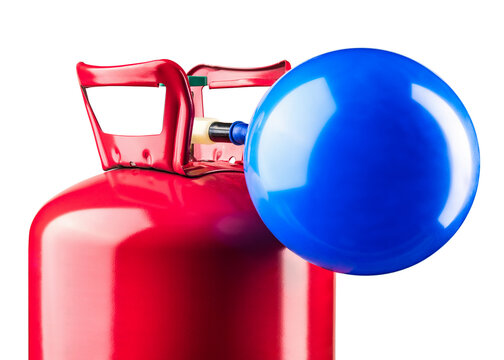
\includegraphics[width=0.3\textwidth,keepaspectratio]{Problem_5/Figs/P5.jpg}
\label{figP5}
\end{figure}

\begin{center}
    \normalcolor{------------------------------------------------ HẾT ------------------------------------------------}
\end{center}

% \newpage
% { \normalcolor \textbf{Danh sách thành viên tham gia xây dựng [Hướng tới chuyên lý 2024]:}} \\ \vspace{0.5cm}

% \textbf{\textit{Thành Viên tham gia đề xuất các bài tập:}}
\begin{enumerate}
    \item \textbf{Hirrus} (Trưởng nhóm)
    \item \textbf{Colevol}
    \item \textbf{Mino}
    \item \textbf{wan}
    \item \textbf{Khui đạp chai}
    \item \textbf{trees\&streetslights.inc}
    \item \textbf{Carina}
    \item \textbf{LunarEclipse}
\end{enumerate}



\end{document}